%% 
%% Copyright 2007-2020 Elsevier Ltd
%% 
%% This file is part of the 'Elsarticle Bundle'.
%% ---------------------------------------------
%% 
%% It may be distributed under the conditions of the LaTeX Project Public
%% License, either version 1.2 of this license or (at your option) any
%% later version.  The latest version of this license is in
%%    http://www.latex-project.org/lppl.txt
%% and version 1.2 or later is part of all distributions of LaTeX
%% version 1999/12/01 or later.
%% 
%% The list of all files belonging to the 'Elsarticle Bundle' is
%% given in the file `manifest.txt'.
%% 
%% Template article for Elsevier's document class `elsarticle'
%% with harvard style bibliographic references

\documentclass[preprint,12pt,authoryear]{elsarticle}

%% Use the option review to obtain double line spacing
%%\documentclass[authoryear,preprint,review,12pt]{elsarticle}

%% Use the options 1p,twocolumn; 3p; 3p,twocolumn; 5p; or 5p,twocolumn
%% for a journal layout:
%% \documentclass[final,1p,times,authoryear]{elsarticle}
%%\documentclass[final,1p,times,twocolumn,authoryear]{elsarticle}
%% \documentclass[final,3p,times,authoryear]{elsarticle}
%% \documentclass[final,3p,times,twocolumn,authoryear]{elsarticle}
%% \documentclass[final,5p,times,authoryear]{elsarticle}
%%\documentclass[final,5p,times,twocolumn,authoryear]{elsarticle}

%% For including figures, graphicx.sty has been loaded in
%% elsarticle.cls. If you prefer to use the old commands
%% please give \usepackage{epsfig}

%% The amssymb package provides various useful mathematical symbols
\usepackage{amssymb}
%% The amsthm package provides extended theorem environments
%% \usepackage{amsthm}

%% The lineno packages adds line numbers. Start line numbering with
%% \begin{linenumbers}, end it with \end{linenumbers}. Or switch it on
%% for the whole article with \linenumbers.
%% \usepackage{lineno}
\usepackage{amsmath}
\usepackage{pgfplotstable,filecontents}
\usepackage{hyperref}
\usepackage{amsmath}
\usepackage{placeins}  % for \FloatBarrier
\usepackage{svg}
\usepackage{caption}
\usepackage{subcaption}
%\usepackage{cancel}
\usepackage{flafter}  % no figures before reference
%\usepackage{layouts}
\usepackage{bm}  % bold text

\journal{International Journal of Naval Architecture and Ocean Engineering}

\begin{document}

\begin{frontmatter}

    %% Title, authors and addresses

    %% use the tnoteref command within \title for footnotes;
    %% use the tnotetext command for theassociated footnote;
    %% use the fnref command within \author or \affiliation for footnotes;
    %% use the fntext command for theassociated footnote;
    %% use the corref command within \author for corresponding author footnotes;
    %% use the cortext command for theassociated footnote;
    %% use the ead command for the email address,
    %% and the form \ead[url] for the home page:
    %% \title{Title\tnoteref{label1}}
    %% \tnotetext[label1]{}
    %% \author{Name\corref{cor1}\fnref{label2}}
    %% \ead{email address}
    %% \ead[url]{home page}
    %% \fntext[label2]{}
    %% \cortext[cor1]{}
    %% \affiliation{organization={},
    %%            addressline={}, 
    %%            city={},
    %%            postcode={}, 
    %%            state={},
    %%            country={}}
    %% \fntext[label3]{}

    %\title{System identification of a physics-informed ship model for better predictions in wind conditions}
    %\title{Virtual Captive Tests for Identifying System-Based Manoeuvring Models}
    \title{Virtual captive tests for standard ship manoeuvres}
    

    %% use optional labels to link authors explicitly to addresses:
    %% \author[label1,label2]{}
    %% \affiliation[label1]{organization={},
    %%             addressline={},
    %%             city={},
    %%             postcode={},
    %%             state={},
    %%             country={}}
    %%
    %% \affiliation[label2]{organization={},
    %%             addressline={},
    %%             city={},
    %%             postcode={},
    %%             state={},
    %%             country={}}

    \author[1,2]{Martin Alexandersson\corref{cor1}%
        %\fnref{fn1,fn3}
    }
    \ead{maralex@chalmers.se}
    \author[1]{Wengang Mao}
    \author[1]{Jonas W. Ringsberg}
    \author[2]{Martin Kjellberg}


    \affiliation[1]{organization={Dept. of Mechanics and Maritime Sciences, Division of Marine Technology, Chalmers University of Technology},%Department and Organization
        addressline={Hörsalsvägen 7A},
        city={Gothenburg},
        postcode={41296},
        country={Sweden}}


    \affiliation[2]{organization={Research Institutes of Sweden (RISE), SSPA Maritime Center},%Department and Organization
        addressline={Chalmers tvärgata 10},
        city={Gothenburg},
        postcode={41296},
        country={Sweden}}

    \cortext[cor1]{Corresponding author}

    \begin{abstract}
        Ships with wind-assisted propulsion systems (WAPS) should be equipped with large rudders to compensate for WAPS-induced drifting forces. The WAPS also significantly affects the effectiveness of mathematical models used to describe the ship's maneuvering characteristics. In this study, the Maneuvering Modeling Group (MMG) is chosen and various approaches are proposed to identify different parameters within the MMG model. First, the ship's hydrodynamic coefficients, such as mass, added mass, and center of gravity, are estimated from either model tests or hydrodynamic analysis. The hydrodynamic forces and drifting forces are proposed to be analyzed by virtual captive tests (VCT). The key part of identifying MMG models for ships with WAPS is to obtain accurate rudder forces. Various explicit semi-empirical formulas are proposed to approximate the rudder forces when experimental data on the rudder forces is not available. Based on the experimental tests with rudder forces measured, the quadratic semi-empirical models are found to perfectly describe such forces. Finally, the other parameters in the MMG model are estimated by the inverse dynamics based on the series of maneuvering tests. In this study, two ships designed with WAPS, i.e., wPCC and Optiwise, are used to validate the proposed method based on their experimental model tests. For the wPCC ship with double rudders, large discrepancies are observed between the close loop maneuvering prediction by the identified model and tests, due to the incapability of VCTs to model rudder forces, and asymmetric patterns of flows on the two rudders. When the measurement of rudder forces is available for the Optiwise ship, the MMG model identified by the proposed method can perfectly predict the ship’s maneuvering motions compared to the tests.
% Move 1 - Background/introduction/situation

% Move 2 - Present research/purpose

% Move 3 - Methods/materials/subjects/procedures

% Move 4 - Results/findings

% Move 5 - Discussion/conclusion/significance

    \end{abstract}

    %%Graphical abstract
    %\begin{graphicalabstract}
    %    %\includegraphics{grabs}
    %\end{graphicalabstract}
    %
    %%%Research highlights
    %\begin{highlights}
    %    \item Research highlight 1
    %    \item Research highlight 2
    %\end{highlights}

    \begin{keyword}
    Inverse dynamics \sep Physics-informed maneuvering model \sep System identification \sep Wind-assisted propulsion 
        %% keywords here, in the form: keyword \sep keyword

        %% PACS codes here, in the form: \PACS code \sep code

        %% MSC codes here, in the form: \MSC code \sep code
        %% or \MSC[2008] code \sep code (2000 is the default)

    \end{keyword}

\end{frontmatter}
%% \linenumbers
%textwidth in inches: \printinunitsof{in}\prntlen{\textwidth} \newline
%textheight in inches: \printinunitsof{in}\prntlen{\textheight}
%% main text
%\newpage
\section*{Nomenclature}
\label{sec:introduction}
\begin{table}[h]
    \centering
    %\footnotesize
    \scriptsize
    %\caption{Semi-empirical rudder parameters (SI units) in model scale.}
    \label{tab:other_parameters}
    \pgfplotstabletypeset[col sep=comma, column type=r,
    columns/LaTeX/.style={column type=r,string type,column name=~},
    columns/LaTeX1/.style={column type=r,string type, column name=~},
    columns/LaTeX2/.style={column type=r,string type, column name=~},
    %columns/LaTeX3/.style={column type=l,string type, column name=~},
    columns/Description/.style={column type=p{3.3cm},string type,column name=~},
    columns/Description1/.style={column type=p{3.3cm},string type, column name=~},
    columns/Description2/.style={column type=p{3.3cm},string type, column name=~},
    %columns/Description3/.style={column type=l,string type, column name=~},
    %every head row/.style={before row=\hline,after row=\hline},
    %every last row/.style={after row=\hline}
    ]{tables/mathematical_model_kinetics.nomenclature.csv}
\end{table}
\FloatBarrier

\section*{Abbreviations}
\label{sec:introduction}
\begin{table}[h]
    \centering
    %\footnotesize
    \scriptsize
    %\caption{Semi-empirical rudder parameters (SI units) in model scale.}
    \label{tab:abbreviations}
    \begin{tabular}{l l}

    CFD & Computational fluid dynamics \\
    CMT & Captive model tests \\
    ID & Inverse dynamics \\
    MMG & Manoeuvring modeling group \\
    OLS & Ordinary least-square \\
    PI model & Physics informed  model \\
    PU model & Physics uninformed  model \\
    RHI & Rudder hull interaction \\
    VCT & Virtual captive tests \\
    WASP & Wind-assisted ship propulsion \\
    wPCC & Wind powered car carrier \\
    SNR & Signal to noise ratio \\
    \end{tabular}
        
\end{table}
\FloatBarrier

\section{Introduction}
\label{sec:introduction}

\section{Results}
\label{sec:results}
%\input{result}
\FloatBarrier

\subsection{Optiwise}
FRMT experiments with Optiwise were conducted as a continuation of the wPCC experiments. During these tests, rudder forces were measured during the experiments, to get a better understanding of the rudder forces during the maneuvers. Prediction models equipped with the semi-empirical rudder, the MMG rudder, or the polynomial rudder were developed. A fourth model was also developed, which uses the actual measured rudder force instead of a prediction model -- so that only the hull forces need to be predicted. 

%10/10
The total forces acting on the ship during the FRMT experiments were estimated with inverse dynamics, in the same way as how the wPCC results were analyzed. There was generally good agreement for the zigzag10/10, as shown in \autoref{fig:ID_optiwise10}. Deviations were however observed for the sway force $Y_D$ during about 3 seconds after the rudder changes at t=11--14 s, and t=35--38 s, as indicated in \autoref{fig:ID_optiwise10}. All of the models and the VCT calculations predict a more straight line in the $Y_D$ time series around these deviation points. 
A reasonable explanation to these deviations has not been found during the work for this paper, where filtration errors in the EKF were ruled out as a possible explanation, by conducting alternative analysis with a low-pass filter instead of the EKF. Accelerations were instead calculated with numeric differentiation of the low-pass filtered signals of repeated zigzag10/10 tests as shown in \autoref{fig:lowpass_deviation_points}.
\begin{figure}[h]
    \centering
    \begin{subfigure}[b]{\textwidth}
        \centering
        \includesvg{figures/results_optiwise_ID.measured_rudder_zigzag 10_10.svg}
        \caption{Zigzag10/10 to port.}
        \label{fig:ID_measured_rudder_zigzag_10_10}
    \end{subfigure}
     \vfill
    \begin{subfigure}[b]{\textwidth}
        \centering
        \includesvg{figures/results_optiwise_ID.measured_rudder_zigzag 20_20.svg}
        \caption{Zigzag20/20 to starboard.}
        \label{fig:ID_measured_rudder_zigzag_20_20}
    \end{subfigure}
    \caption{Inverse dynamics forces during the zigzag tests compared to predictions with the measured rudder model.}
    \label{fig:ID_optiwise20}
\end{figure}
%20/20
The force predictions for the zigzag20/20 is shown in \autoref{fig:ID_optiwise20}. Similar deviations as for the zigzag10/10 were observed for $Y_D$ after the rudder changes (t=11--14 s, t=35--38 s, t=64 s). The yawing moment $N_D$ was not well predicted for the MMG rudder in the end of the port turn (t=23--33 s), where the other models had better agreement with the experiments. When the ship started to turn back to starboard (t=43--62 s) only the measured rudder forces model and the polynomial rudder agreed well with the experiments. Just as for wPCC, the total yawing moment $N_D$ deviations seem to originate from the rudder yawing moment $N_R$ predictions.
\begin{figure}[h]
    \centering
    \includesvg{figures/results_optiwise_deviation_points.lowpass.svg}
    \caption{Inverse dynamics sway force from repeated zigzag10/10 test to port. The accelerations have been estimated with the EKF and also with numeric differentiation of low-pass filtered signals.}
    \label{fig:lowpass_deviation_points}
\end{figure}



%\begin{figure}[h]
%     \centering
%     \begin{subfigure}[b]{\textwidth}
%         \centering
%         \includesvg{figures/results_optiwise_ID.zigzag 10_10.svg}
%        \caption{Forces Optiwise Zigzag10/10 to port.}
%        \label{fig:ID_optiwise10}
%     \end{subfigure}
%     \vfill
%     \begin{subfigure}[b]{\textwidth}
%         \includesvg{figures/results_optiwise_ID.zigzag 20_20.svg}
%        \caption{Forces Optiwise Zigzag20/20 to starboard.}
%        \label{fig:ID_optiwise20}
%     \end{subfigure}
%        \caption{Comparison between forces during zigzag tests with Optiwise estimated with inverse dynamics from the experiments and predictions with a model equipped with either a polynomial rudder or semi-empirical rudder model. Forces from VCT calculations of some interesting states have also been added.}
%        \label{fig:ID_optiwise}
%\end{figure}


The results of closed-loop simulations with the Optiwise simulation model equipped with either the MMG original or the quadratic model are shown in \autoref{fig:sim_optiwise}. There was very good agreement for the zigzag20/20 tests and a little less agreement for the zigzag10/10 tests, where the MMG quadratic was the better of the two models. Up to four degrees of deviation was observed between the overshoot angles, as shown in \autoref{fig:overshoots_optiwise}.   
\begin{figure}[h]
     \centering
     \begin{subfigure}[b]{0.40\textwidth}
         \centering
         \includesvg{figures/results_optiwise_ID.closed loop zigzag 10_10 port.svg}
        \caption{Zigzag10/10 to port.}
        \label{fig:sim_optiwise_10_port}
     \end{subfigure}
     \hfill
     \begin{subfigure}[b]{0.40\textwidth}
         \includesvg{figures/results_optiwise_ID.closed loop zigzag 10_10 stbd.svg}
        \caption{Zigzag10/10 to starboard.}
        \label{fig:sim_optiwise_10_stbd}
     \end{subfigure}
     \vfill
     \begin{subfigure}[b]{0.40\textwidth}
         \centering
         \includesvg{figures/results_optiwise_ID.closed loop zigzag 20_20 port.svg}
        \caption{Zigzag20/20 to port.}
        \label{fig:sim_optiwise_20_port}
     \end{subfigure}
     \hfill
     \begin{subfigure}[b]{0.40\textwidth}
         \includesvg{figures/results_optiwise_ID.closed loop zigzag 20_20 stbd.svg}
        \caption{Zigzag20/20 to starboard.}
        \label{fig:sim_optiwise_20_stbd}
     \end{subfigure}
     
        \caption{Comparison of zigzag tests between experiments and simulations with the MMG rudder models.}
        \label{fig:sim_optiwise}
\end{figure}
\vspace{-1cm}

\begin{figure}[b!]
    \centering
    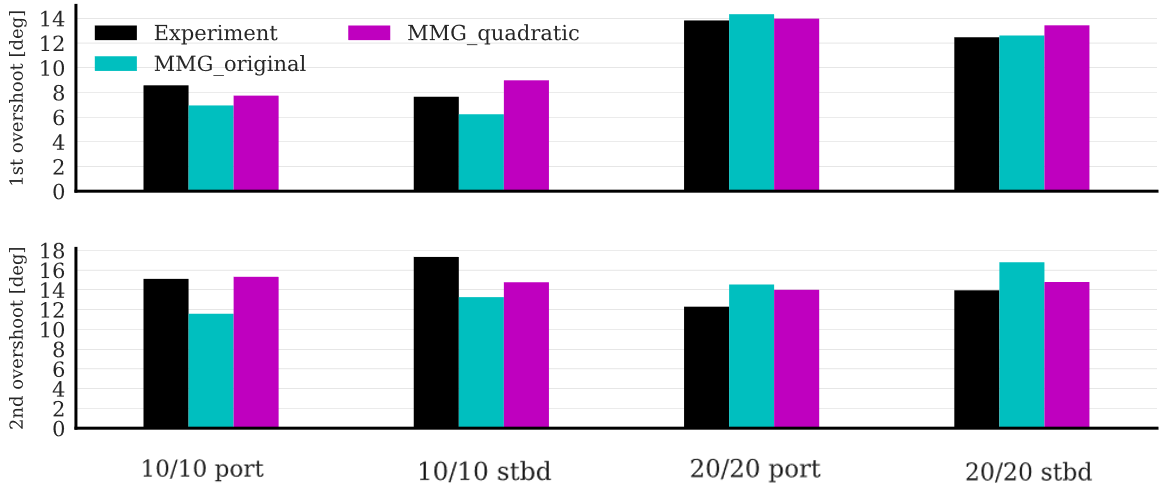
\includegraphics[width=0.9\linewidth, height = 5cm]{figures/results_optiwise_overshoot.png}
    \caption{Overshoot angles from the Optiwise experiments and simulations.}
    \label{fig:overshoots_optiwise}
\end{figure}
\vspace{-0.5cm}
% \begin{figure}[h]
%      \centering
%      \begin{subfigure}[b]{\textwidth}
%          \centering
%          \includesvg{figures/results_optiwise_ID.overshoot1.svg}
%         \caption{First overshoot angles.}
%         \label{fig:overhoots1_optiwise}
%      \end{subfigure}
%      \vfill
%      \begin{subfigure}[b]{\textwidth}
%          \centering
%          \includesvg{figures/results_optiwise_ID.overshoot2.svg}
%         \caption{Second overshoot angles.}
%         \label{fig:overhoots2_optiwise}
%      \end{subfigure}
     
%         \caption{Overshoot angles from the Optiwise experiments and simulations.}
%         \label{fig:overshoots_optiwise}
% \end{figure}
\FloatBarrier

\subsection{Inverse dynamics wPCC}
Forces predicted with the wPCC model equipped with either the semi-empirical rudder or the polynomial rudder have been compared with forces from the experiment, estimated by inverse dynamics. Both rudder models have reasonably good agreement with the experimental results from the zigzag10/10 test (see \autoref{fig:ID_wPCC_10}). For the 20/20 test, only the polynomial rudder model seems to capture the forces correctly (see \autoref{fig:ID_wPCC_20}). There are however some yawing moment $N_D$ deviations during the rudder transitions at t=9.5 s, and t=27 s.

\begin{figure}
     \centering
     \begin{subfigure}[b]{\textwidth}
         \centering
         \includesvg{figures/results_wPCC_ID.zigzag 10_10.svg}
        \caption{Zigzag10/10 to port.}
        \label{fig:ID_wPCC_10}
     \end{subfigure}
     \vfill
     \begin{subfigure}[b]{\textwidth}
         \includesvg{figures/results_wPCC_ID.zigzag 20_20.svg}
        \caption{Zigzag20/20 to starboard.}
        \label{fig:ID_wPCC_20}
     \end{subfigure}
        \caption{Comparison between forces during zigzag tests estimated with inverse dynamics from the experiments and predictions with a model equipped with either a polynomial rudder or semi-empirical rudder model. Forces from VCT calculations of some interesting states have also been added.}
        \label{fig:ID_wPCC}
\end{figure}
\FloatBarrier

\section{Discussion}
\label{sec:discussion}


\section{Conclusions}
\label{sec:conclusions}
%_________________________________________________________
%Move 1: Background information (research purposes, theory,
%methodology)
%
\noindent Maneuvering models were developed for two WAPS test cases with large rudders. The models were identified by conducting VCTs to obtain the hydrodynamic damping coefficients and by conducting pure yaw and pure sway simulations in the FNPF to obtain the added masses. The identified force models were compared with the inverse dynamics forces of the zigzag tests to identify possible weak spots within the models.  

%%_________________________________________________________
%%Move 2: Summarizing and reporting key results. (oblig.)
The identified wPCC model was shown to be well adapted to the VCT data, where the importance of the coupling terms was also shown in the combined drift and yaw rate cases.
However, the FRMT inverse dynamics forces were quite different from the VCT data and the model predictions. From this it was concluded that there must be an inherent error in the VCT data for wPCC that was inherited by the identified hull force model.

The inherent error in the wPCC VCT data could originate from false assumptions about neglected wave generation and roll exclusion. Therefore, another test case, Optiwise, was investigated in which these assumptions were assumed to be more valid.

It was shown that a model, with the rudder model replaced by the actual measured rudder forces, predicted total forces that were similar to the total forces from the inverse dynamics. Hence, it was concluded that for Optiwise the hull force prediction was correct.

The newly proposed MMG quadratic rudder model was then shown to be identifiable from the VCT data to get good agreement, in fact even better than the original MMG rudder model, with the FRMT measured rudder forces and consequently also good agreement with the total forces. 
%_________________________________________________________
%Move 3: Commenting on key results (making claims, explaining the results,
%comparing the new work with previous studies, offering
%alternative explanations) (oblig.)
For Optiwise it can be concluded that the VCT data contained correct damping forces during the maneuvers, which were well described by the chosen model structure, and also that the method used to determine added masses gave reasonable values. 

This analysis of the wPCC and Optiwise test cases has shown that inverse dynamics together with state VCTs is an effective tool to identify and explain possible weak spots within the identified models.

%It was shown that the proposed way to determine added masses with FNPF pure yaw and pure sway tests
%
%added masses from the FNPF pure yaw and pure sway tests produced inverse dynamics forces that agreed well with the force prediction models and the state VCTs for the Optiwise test case, which suggests that this is an accurate way to determine the added masses.
%
%Two enhancements to the MMG rudder model were proposed which improved the fit to the VCT data and also gave a little bit better results in the closed loop simulations.
%The coupling terms between sway and yaw rate were important for both wPCC and Optiwise.

%_________________________________________________________
%Move 4: Stating the limitations of the study
It should also be mentioned that if completely new maneuvers are simulated, the models in this paper would need a propeller prediction model that would be self-containing.
%_________________________________________________________
%Move 5: Making recommendations for future implementation and/or for
%future research

\FloatBarrier

\section{Acknowledgements}
\noindent The authors would like to acknowledge Trafikverket (Swedish Transport Administration) and Lighthouse, swedish maritime competence centre (www.lighthouse.nu) for providing the resources to prepare this paper. They would also thank all personnel at SSPA Maritime Center who have been involved in creating the model test results, building the ship models, and conducting the experiments.

%% The Appendices part is started with the command \appendix;
%% appendix sections are then done as normal sections
\appendix


\FloatBarrier
%% If you have bibdatabase file and want bibtex to generate the
%% bibitems, please use
%%
\pagebreak
\bibliographystyle{elsarticle-harv}
\bibliography{Paper_3_semiempirical_rudder.bib}

\end{document}

\endinput
%%
%% End of file `elsarticle-template-harv.tex'.
